\documentclass[a4paper]{article}

\usepackage[]{authblk}
\usepackage{graphicx}
\usepackage{tikz}

\graphicspath{ {./figs/} }

\title{The ILD simulation model in lcgeo (DD4hep) }

%\author{Frank Gaede$^{a,b}$ \\ % E-mail: {frank.gaede@desy.de}
%  \footnotesize
%  $^a$~Deutsches-Elektronen-Synchrotron, DESY, Notkestr.85, 22607 Hamburg, Germany\\
%  $^b$~CERN, Route de Meyrin 385, 1217 Meyrin, Switzerland
%} 
\author{Frank Gaede, DESY \\ % E-mail: {frank.gaede@desy.de}
%  Deutsches-Elektronen-Synchrotron, DESY, Notkestr.85, 22607 Hamburg, Germany
}
\date{\today}

%1234567890123456789012345678901234567890123456789012345678901234567890123456789


\begin{document}

\maketitle
%\abstract{This document describes the ILD simulation model in lcge (DD4hep)... }
%=============================================================================
%\tableofcontents 
%=============================================================================

\section{Envelopes}
The new ILD simulation model has mandatory envelope volumes defined for the individual subdetectors.
This section describes the current parameters for these envelope volumes and their shapes.


{\small
  \begin{table}
    \documentclass[a4]{article}
\usepackage{multirow}
\usepackage[a4paper,top=3cm, bottom=2.5cm, left=1cm, right=2cm ]{geometry}
\begin{document}
\begin{tabular}{|l | c | c | c | l r |}
\hline
\multicolumn{6}{|c|}{} \\
\multicolumn{6}{|c|}{\large{Envelope parameters for ILD\_o1\_v05}} \\
\multicolumn{6}{|c|}{} \\
\hline
 detector & inner radius & outer radius & half length  & \multicolumn{2}{c|}{additional parameters} \\
          &              &              & min z, max z &          &        \\
\hline
VXD & 16.0 & 60.0 & 177.6 & \small{\verb#VXD_cone_min_z#} & 80.0  \\ 
 & & & & \small{\verb#VXD_cone_max_z#} & 150.0  \\ 
 & & & & \small{\verb#VXD_inner_radius_1#} & 24.1  \\ 
\hline
FTD & 25.1 & 328.9 & 2350.0 & \small{\verb#FTD_outer_radius_1#} & 152.8  \\ 
 & & & & \small{\verb#FTD_outer_radius_2#} & 299.7  \\ 
 & & & & \small{\verb#FTD_min_z_0#} & 177.7  \\ 
 & & & & \small{\verb#FTD_min_z_1#} & 368.2  \\ 
 & & & & \small{\verb#FTD_min_z_2#} & 644.2  \\ 
 & & & & \small{\verb#FTD_cone_min_z#} & 230.0  \\ 
 & & & & \small{\verb#FTD_cone_radius#} & 184.1  \\ 
\hline
SIT & 152.9 & 324.6 & 644.1 & \small{\verb#SIT_outer_radius_1#} & 299.8  \\ 
 & & & & \small{\verb#SIT_half_length_1#} & 368.1  \\ 
\hline
TPC & 329.0 & 1808.0 & 2350.0 &  &   \\ 
\hline
SET & 1808.1 & 1827.9 & 2350.0 &  &   \\ 
\hline
Ecal & 1843.0 & 2028.0 & 2350.0 & \small{\verb#Ecal_Hcal_symmetry#} & 8.0  \\ 
 & & & & \small{\verb#Ecal_symmetry#} & 8.0  \\ 
\hline
EcalEndcap & 400.0 & 2088.8 & 2450.0, 2635.0 &  &   \\ 
\hline
EcalEndcapRing & 250.0 & 390.0 & 2450.0, 2635.0 &  &   \\ 
\hline
Hcal & 2058.0 & 3395.5 & 2350.0 & \small{\verb#Hcal_inner_symmetry#} & 8.0  \\ 
\hline
HcalEndcap & 350.0 & 3395.5 & 2670.7, 3957.7 & \small{\verb#EcalEndcap_symmetry#} & 8.0  \\ 
\hline
HcalEndcapRing & 2138.8 & 3137.0 & 2450.0, 2635.0 & \small{\verb#HcalEndcapRing_symmetry#} & 8.0  \\ 
\hline
Coil & 3425.0 & 4175.0 & 3872.0 &  &   \\ 
\hline
Yoke & 4424.0 & 7725.0 & 4047.0 & \small{\verb#Yoke_symmetry#} & 12.0  \\ 
\hline
YokeEndcap & 300.0 & 7725.0 & 4072.0, 7373.0 & \small{\verb#YokeEndcap_symmetry#} & 12.0  \\ 
\hline
YokeEndcapPlug & 300.0 & 3395.5 & 3981.5, 4072.0 & \small{\verb#YokeEndcapPlug_symmetry#} & 12.0  \\ 
\hline
BeamCal & 20.0 & 150.0 & 3475.0, 3695.0 & \small{\verb#BeamCal_thickness#} & 220.0  \\ 
 & & & & \small{\verb#BeamCal_tubeIncoming_radius#} & 15.0  \\ 
\hline
LHCal & 100.0 & 325.0 & 2680.0, 3200.0 & \small{\verb#LHCal_thickness#} & 520.0  \\ 
\hline
LumiCal & 80.0 & 195.2 & 2500.0, 2630.7 & \small{\verb#LumiCal_thickness#} & 130.7  \\ 
\hline
\end{tabular}
\end{document}

    \caption{Parameters of the envelope volumes in the simulation model. 
      \em{Note: inner and outer radii describe the inscribing cylinder for regular polyhedral barrel detectors.}
      See Fig.\ref{ild:fig:rphi_envelopes} for the symmetries of the barrel envelopes.
    }

  \end{table}
}

\begin{figure}[th]
  \centering
  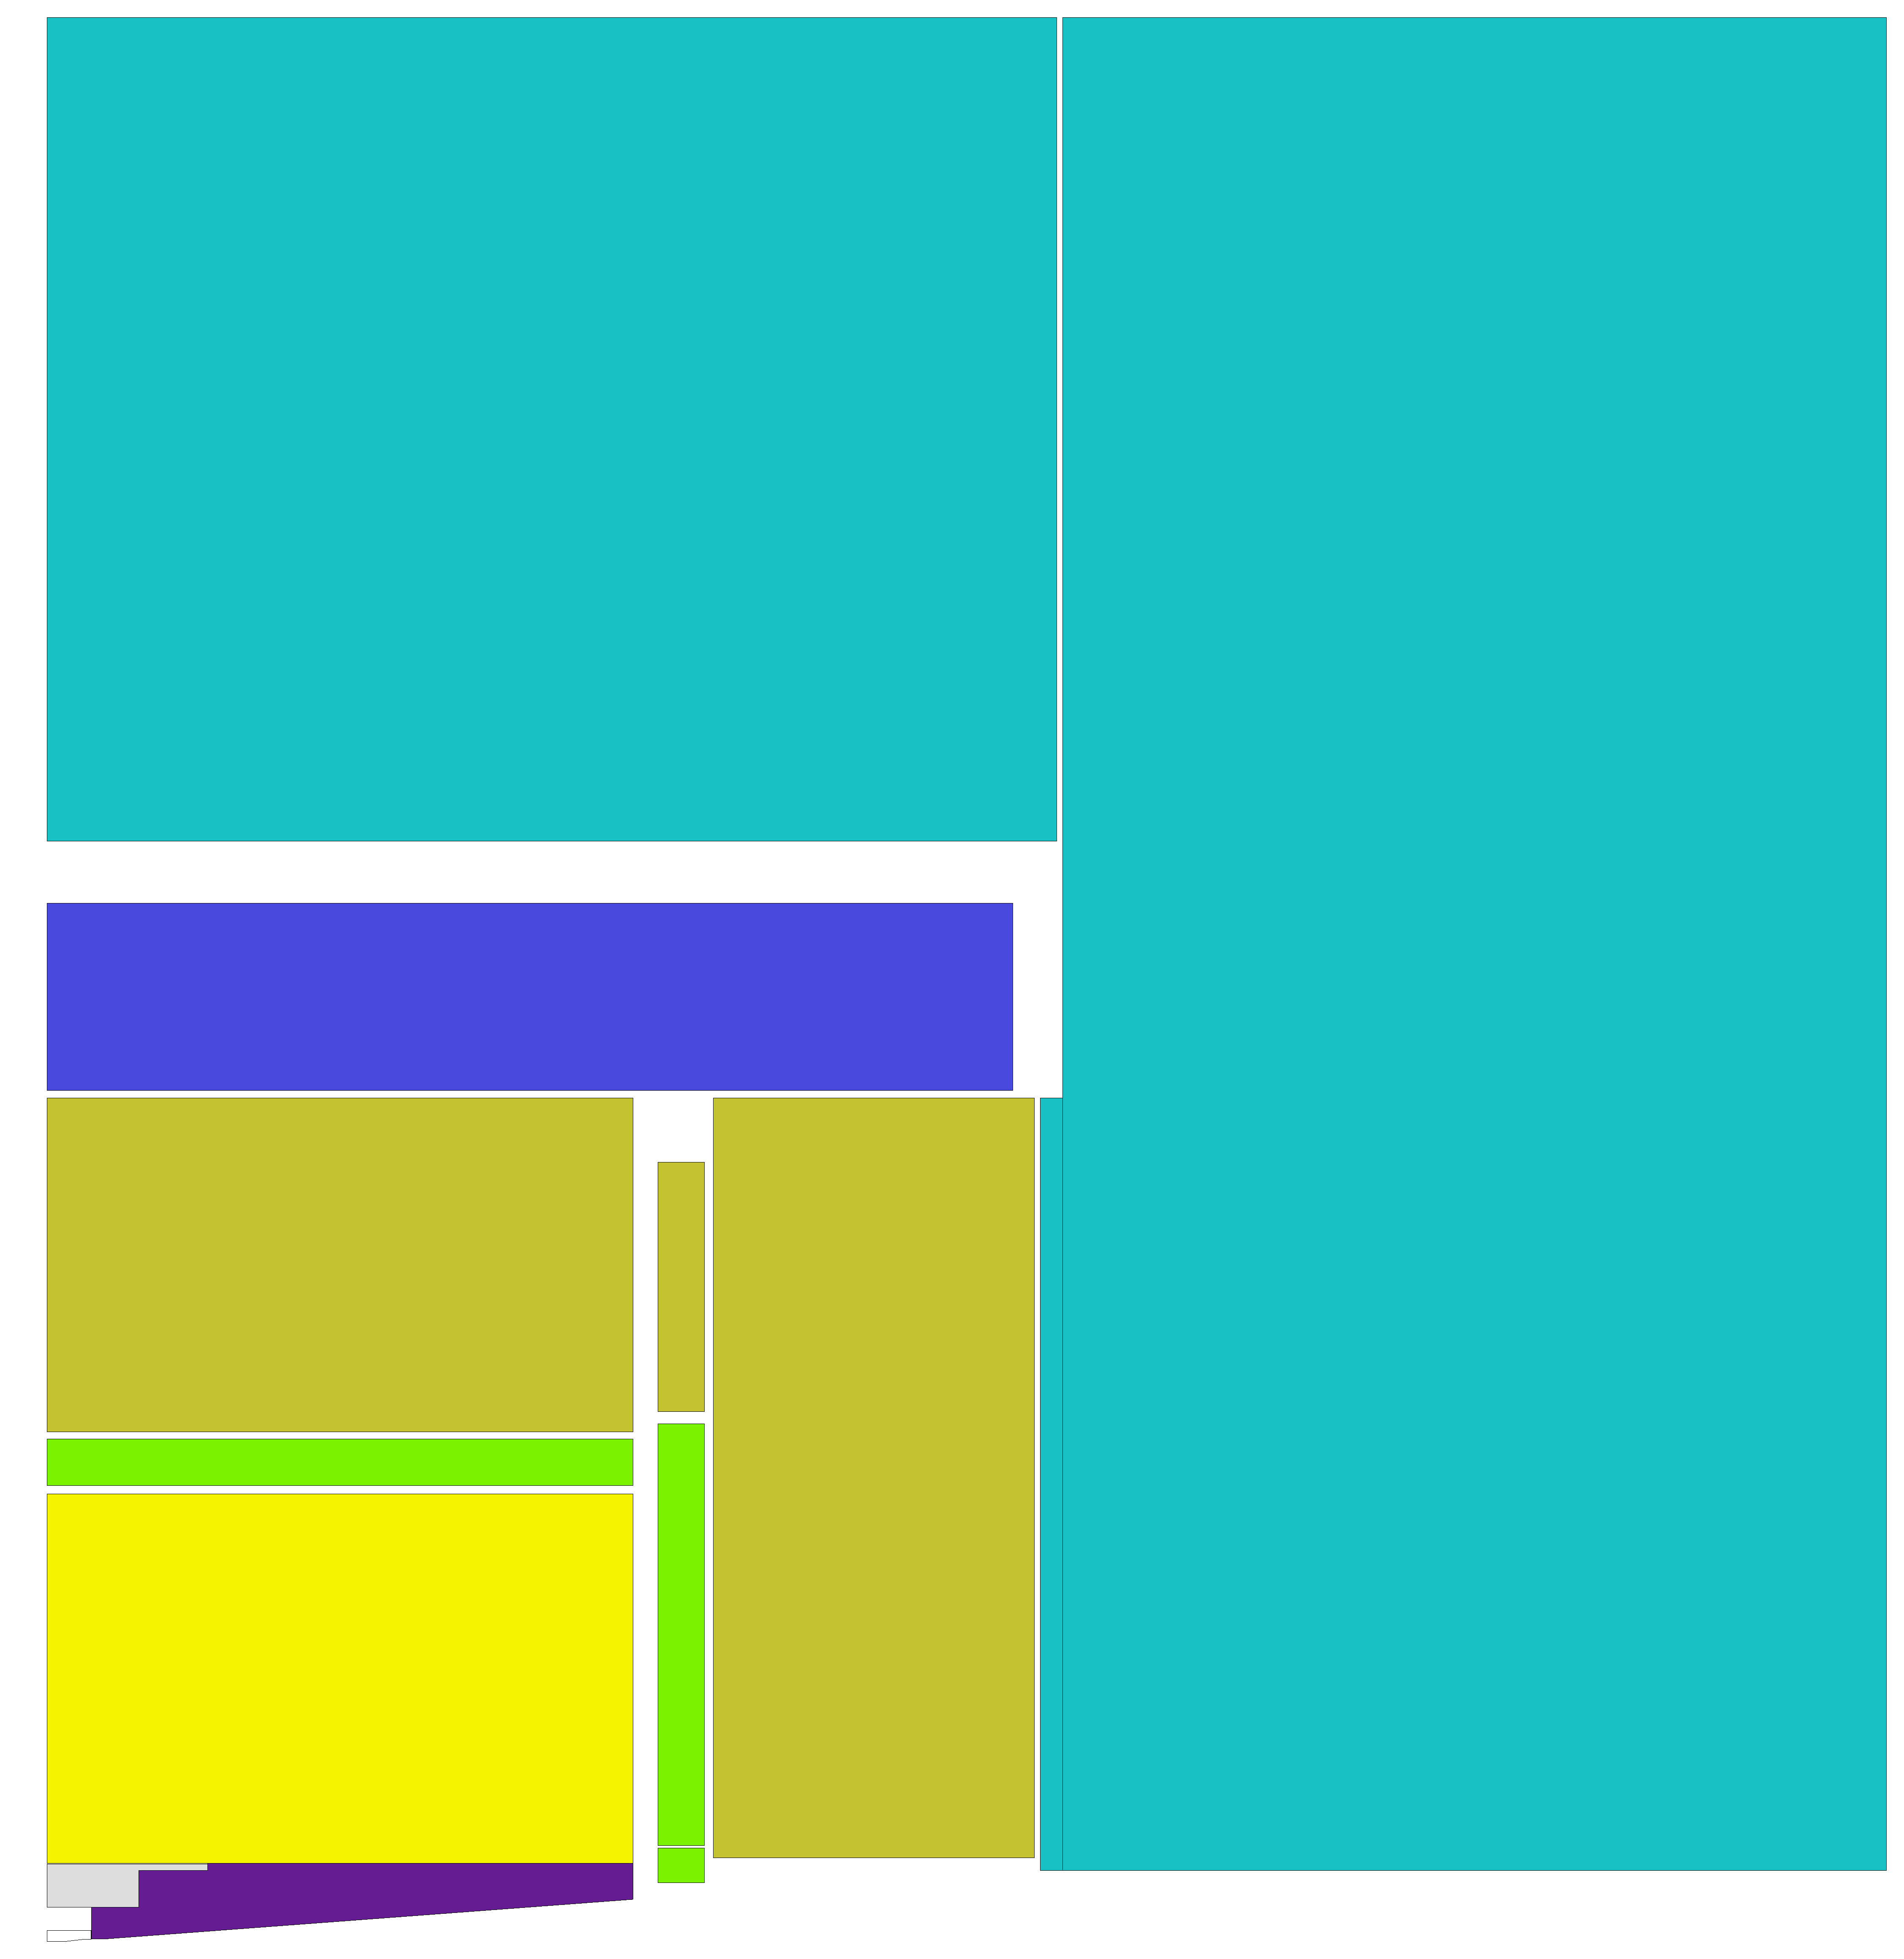
\includegraphics[width=\columnwidth]{ILD_rz_quadrant}
  \caption{Envelope volumes for ILD detectors in simulation model}
  \label{ild:fig:rz_envelopes}
\end{figure}

\begin{figure}[th]
  \centering
  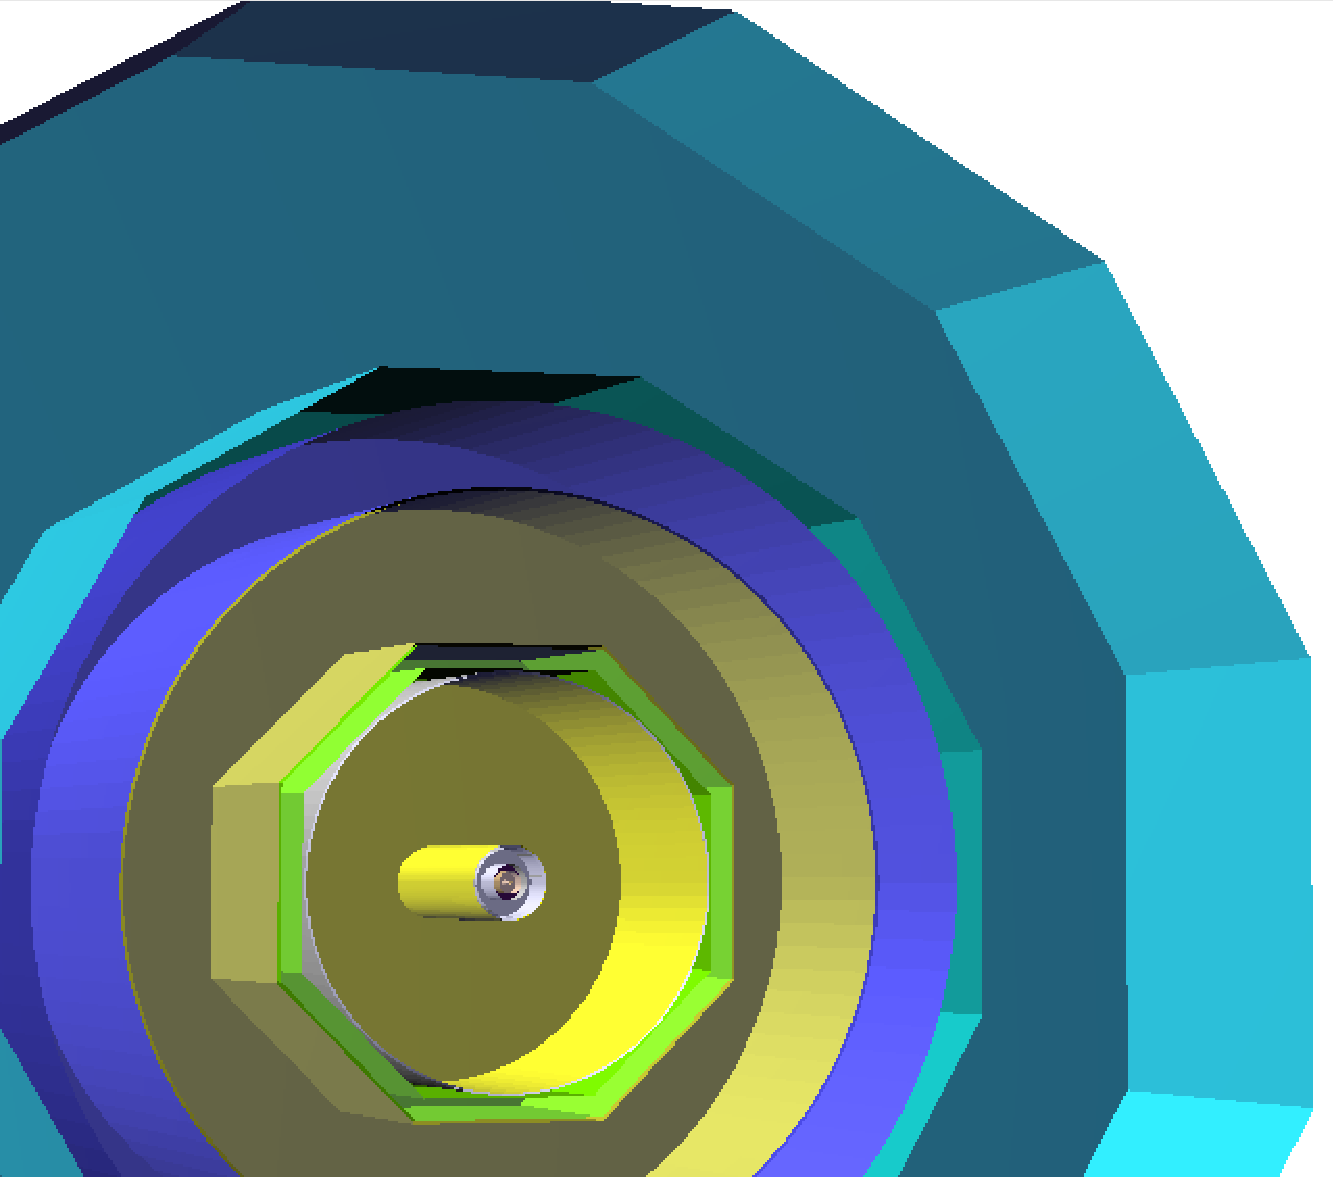
\includegraphics[width=\columnwidth]{ILD_envelopes_3d_front}
  \caption{Barrel envelope volumes for ILD detectors in simulation model as seen from the front}
  \label{ild:fig:rphi_envelopes}
\end{figure}

\begin{figure}[th]
  \centering
  \includegraphics[width=\columnwidth]{tracking_envelopes}
  \caption{Envelopes for the tracking detectors in ILD: VXD, SIT, FTD, TPC, SET.}
  \label{ild:fig:trk_envelopes}
\end{figure}


\begin{figure}[th]
  \centering
  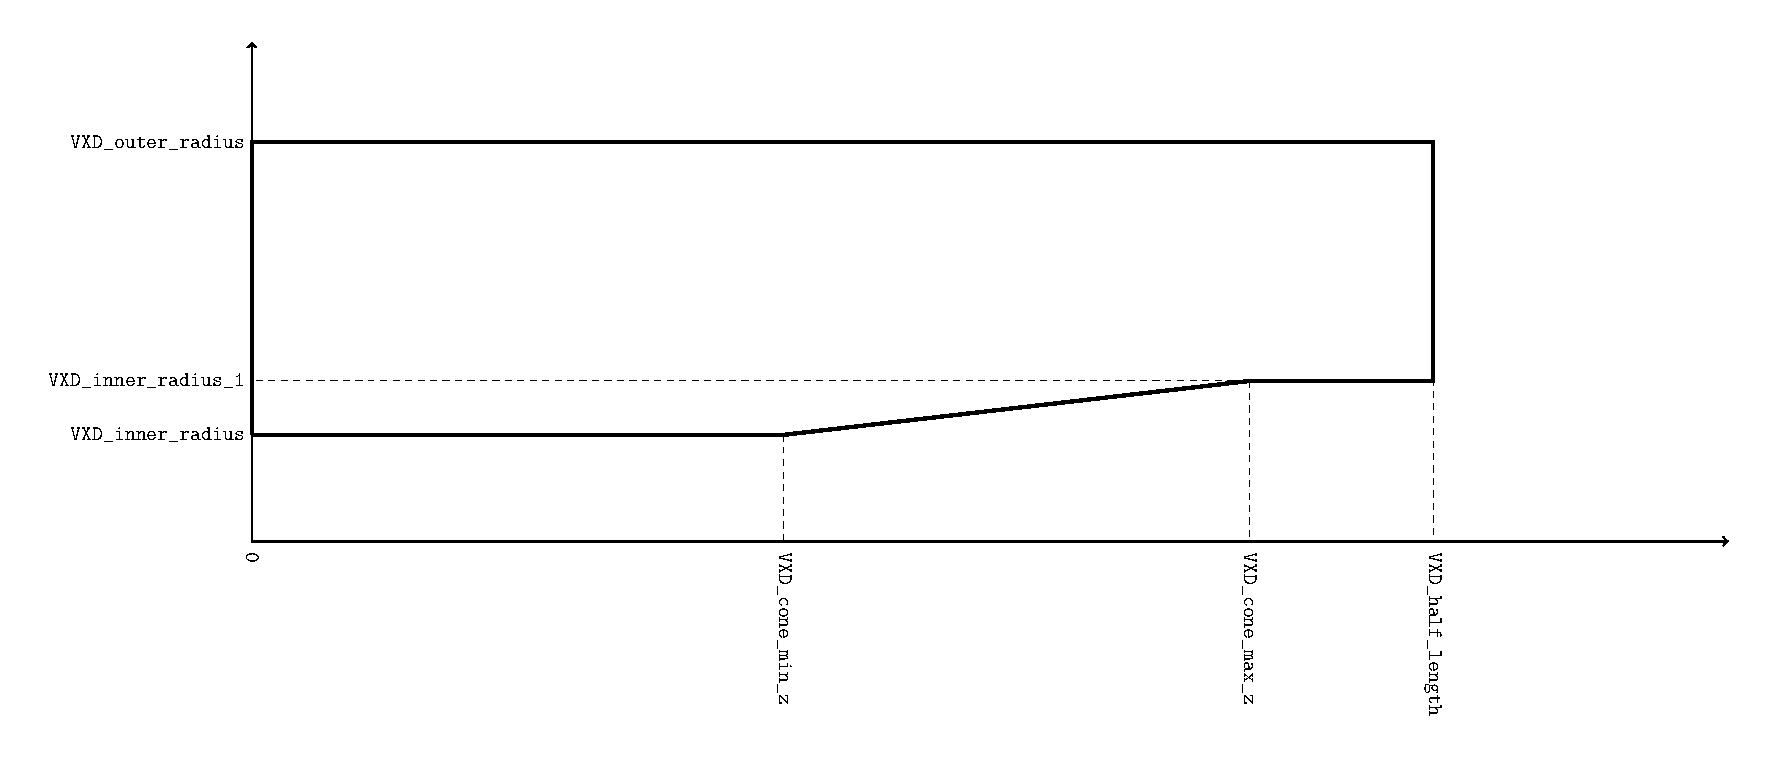
\includegraphics[width=1.3\columnwidth]{VXD_rz_envelope}
  \caption{side view of the VXD envelope}
  \label{ild:fig:vxd_env_rz}
\end{figure}

\begin{figure}[th]
  \centering
  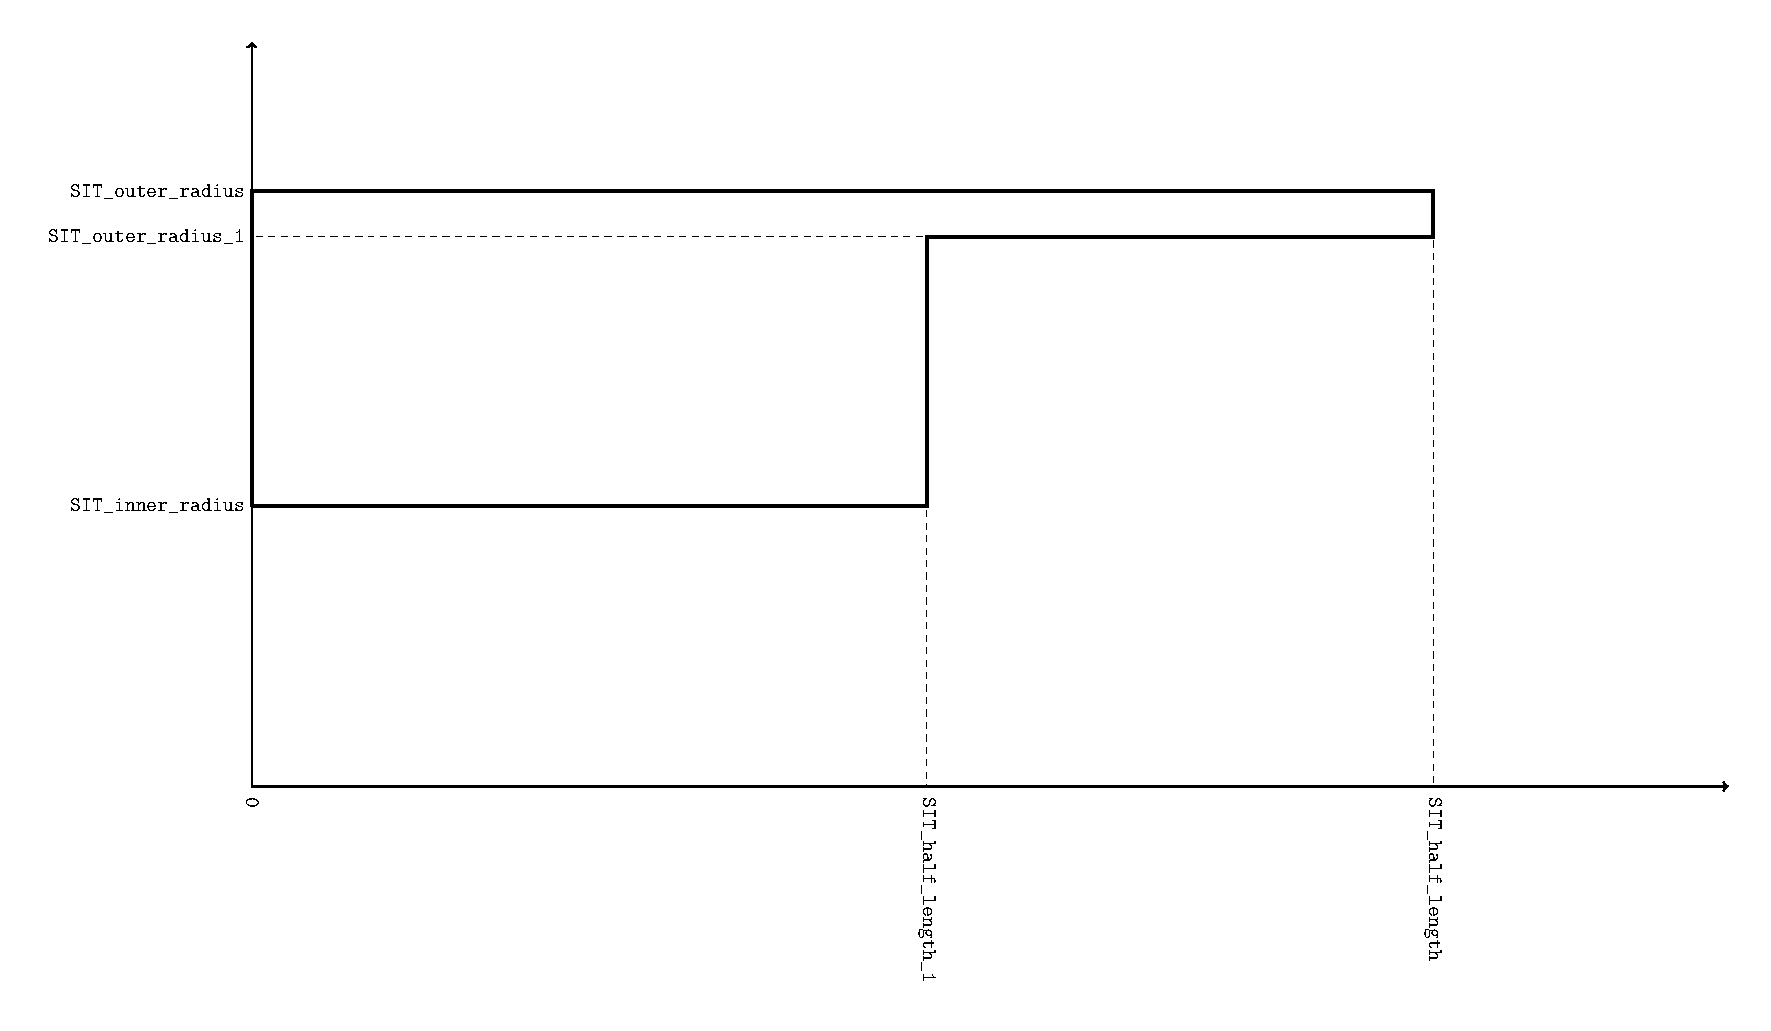
\includegraphics[width=1.3\columnwidth]{SIT_rz_envelope}
  \caption{side view of the SIT envelope}
  \label{ild:fig:sit_env_rz}
\end{figure}

\begin{figure}[th]
  \centering
  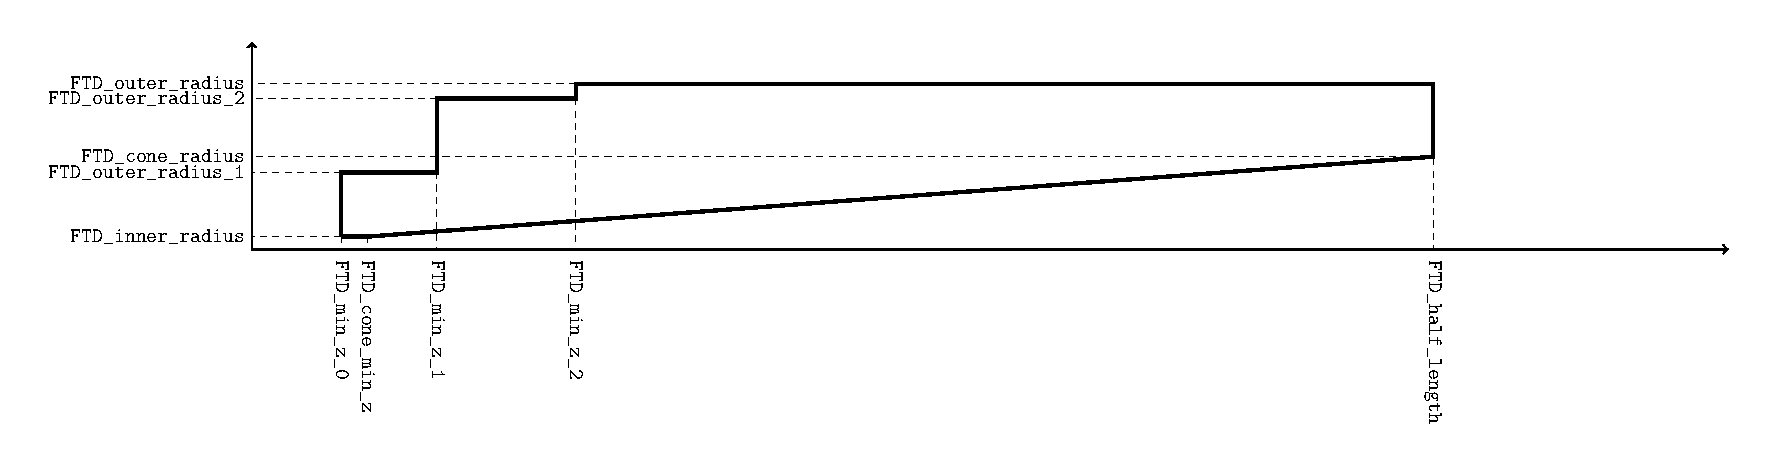
\includegraphics[width=1.3\columnwidth]{FTD_rz_envelope}
  \caption{side view of the FTD envelope}
  \label{ild:fig:ftd_env_rz}
\end{figure}

\begin{figure}[th]
  \centering
  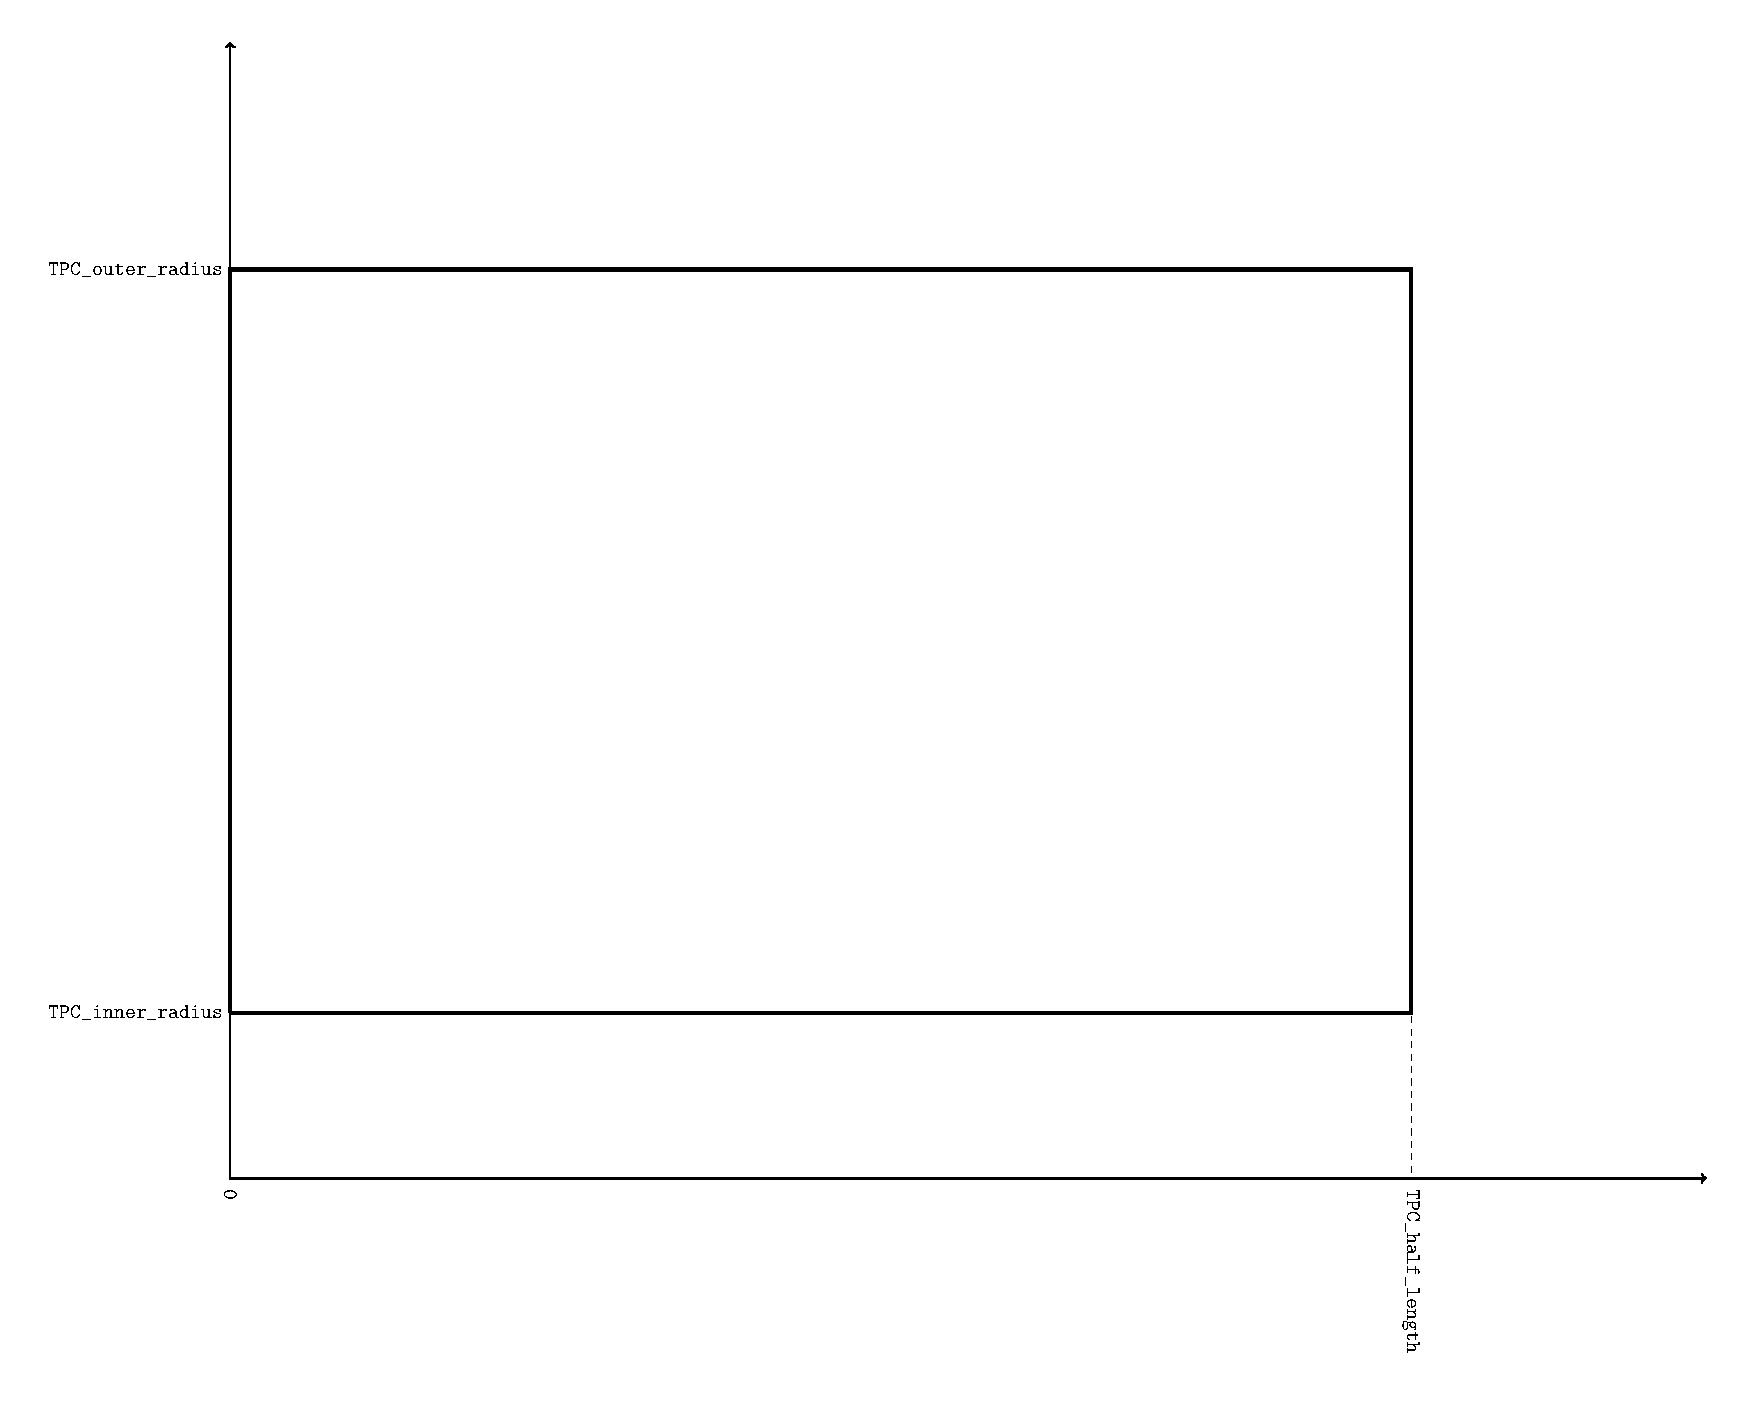
\includegraphics[width=\columnwidth]{TPC_rz_envelope}
  \caption{side view of the TPC envelope}
  \label{ild:fig:tpc_env_rz}
\end{figure}

\begin{figure}[th]
  \centering
  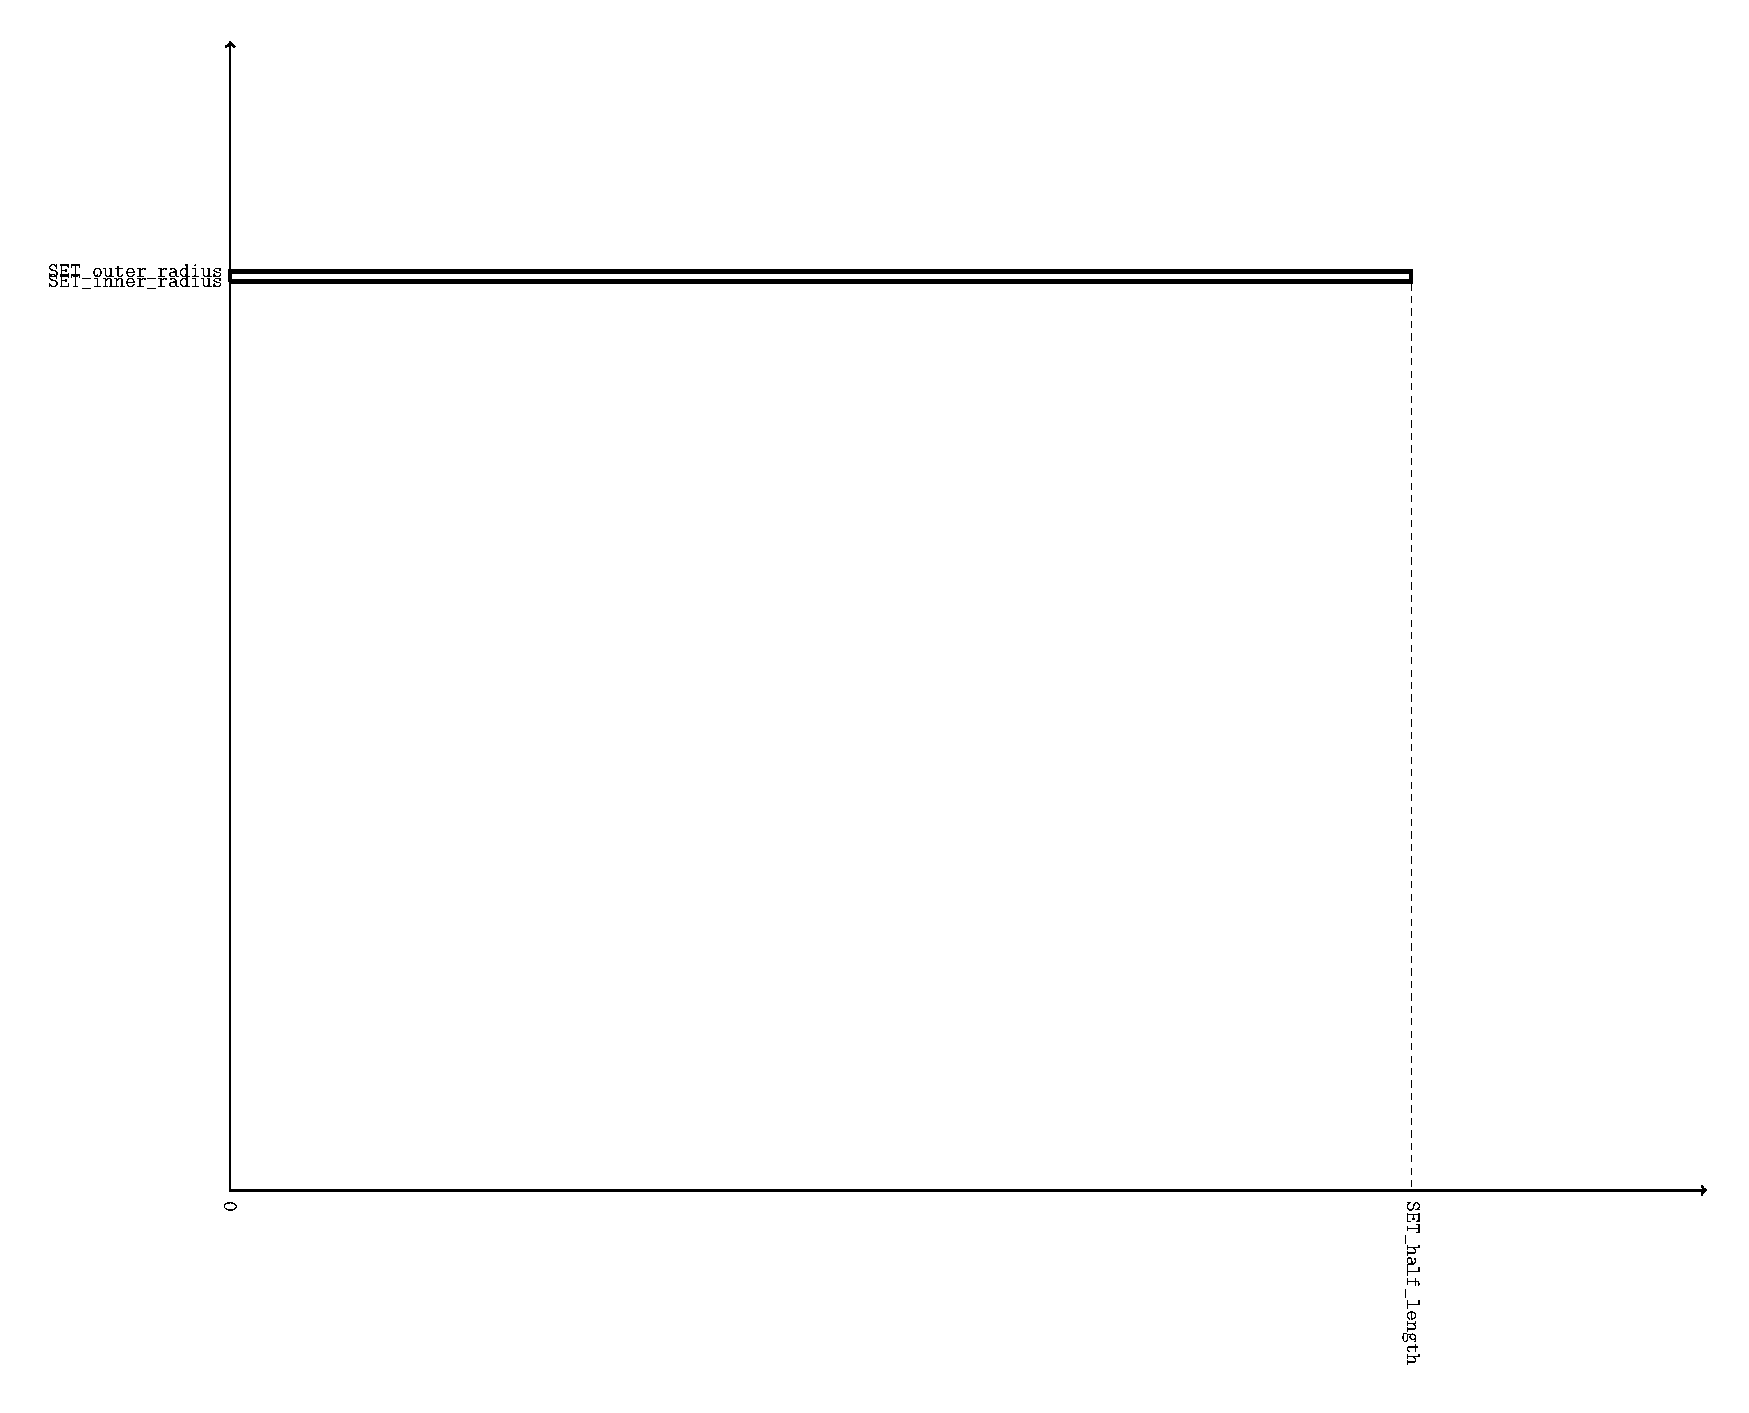
\includegraphics[width=1.3\columnwidth]{SET_rz_envelope}
  \caption{side view of the SET envelope}
  \label{ild:fig:set_env_rz}
\end{figure}


%\section{Summary and Outlook}



%%============================================================================
%% References
%%============================================================================


%\bibliographystyle{plain}
%\bibliography{ILD-simulation}


\end{document}
